It is more useful to know how much time is left until the release in `people hours' instead of CPU hours. In reality, every CPU hour of testing may take a while longer, since it requires the testing team to prepare the data, generate a random input and verify the output. Suppose that every CPU hour requires 2.5 people hours and that the testing team consists of 2 people. Hence, every CPU hour costs the company 1.25 people hours. Furthermore, suppose that for every failure an additional 1.5 hours are required to verify it and write a report for the repair team. So it takes 0.75 hours per failure per person. So the expected time spent reporting and verifying failures for a CPU hour of testing is 0.75 times the expected number of failures in an hour. We have shown in Section \ref{sec:2.2} that given $M(t_e)=m_e$ the expected number of bugs in $[t_e,\tau)$ is given by
$$
    \Tilde{\mu}(\tau) = \int_0^{\tau} (u-m_e)\lambda(t_e+t\mid M(t_e)=m_e)\,dt=\int_0^{\tau}(u-m_e)\frac{f(t_e+t)}{1-F(t_e)}\,dt.
$$
Using $F(t)=1-e^{-\beta t}$ and $f(t)=\beta e^{-\beta t}$ we get that
$$
\Tilde{\mu}(\tau) = \int_0^\tau (u-m_e)\frac{\beta e^{-\beta(t_e+t)}}{e^{-\beta t_e}}\,dt=(1-e^{-\beta\tau})(u-m_e)
$$
and we can substitute the estimators found in Section \ref{sec:estimators} (note that $\beta$ was stated in CPU seconds, but we can simply divide by 3600 to convert it to hours). Then
$$
\nu_t(\tau) = 1.25\tau+0.75\Tilde{\mu}(\tau)
$$
is the number of people hours it takes the test team for $\tau$ CPU hours.

Moving to the repair team, they are only needed whenever there's a failure. Assuming that the repair team takes 6 people hours per bug (for one person) and consists of 2 people we get that
$$
\nu_r(\tau)=3\Tilde{\mu}(\tau)
$$
Lastly we consider the computers needed. We assume that for every CPU hour the computer runs for 6 hours (running external libraries and background processes). Additionally we assume that every failure costs an additional 0.5 hours. Assuming that 4 computers are available full time we get
$$
\nu_c(\tau) = 1.5\tau+0.125\Tilde{\mu}(\tau)
$$
\begin{figure}
    \centering
    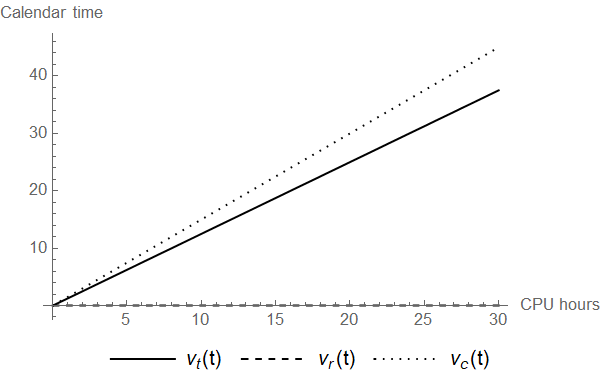
\includegraphics[width=10cm]{img/plot.png}
    \caption{Calendar time vs CPU time for the three teams}
    \label{fig:plot}
\end{figure}

At this point we stop for a moment to check that our model thus far makes intuitive sense. According to our estimates the testing team at MathWorks found over 95\% of the bugs in the software. Therefore the repair team has little work left to do and most of the testing time is spent on generating inputs and verifying outputs. Thus the computers running the software will consume the most time, as seen from Figure \ref{fig:plot}. 

The total time that passes during the interval $(0, \tau]$ (where $\tau$ is in CPU hours) depends on the load on each team. We assume that the teams are called upon simultaneously which is approximately true. At any given moment, any of the three groups might be the limiting factor. When testing starts, many bugs are discovered rapidly and the testing needs to stop often to give the repair team sufficient time to fix the bugs. Hence they will be the limiting factor. But as the failures become more sparse, the repair team has less to do and ultimately the computer resources (how fast can they test different outputs) become the limiting factor. In any given interval, the team that is the limiting factor is the one that has the highest increase in people hours compared to CPU hours. In other words, the graph with the steepest slope. Hence the amount of people hours elapsed after $\tau$ CPU hours is given by
\begin{align*}
    \nu(\tau) &= \int_0^\tau \max\{v_t'(t), v_r'(t), v_c'(t)\}\,dt
\end{align*}
where
\begin{align*}
    \nu_t'(t)&=-0.75 \beta  e^{\beta  (-t)} \left(e^{\beta  t}-1\right) \left(u-m_e\right)+0.75 \beta  \left(u-m_e\right)+1.25,\\
    \nu_r'(t)&=3 \beta  \left(u-m_e\right)-3 \beta  e^{\beta  (-t)} \left(e^{\beta  t}-1\right) \left(u-m_e\right)\\
    \text{and}\\
    \nu_c'(t)&=-0.125 \beta  e^{\beta  (-t)} \left(e^{\beta  t}-1\right) \left(u-m_e\right)+0.125 \beta  \left(u-m_e\right)+1.5.
\end{align*}

\begin{figure}
    \centering
    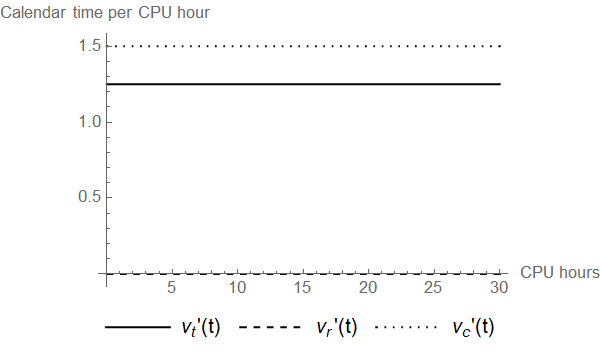
\includegraphics[width=10cm]{img/dplot.png}
    \caption{Calendar time per CPU time for the three teams}
    \label{fig:dplot}
\end{figure}

We know from Section \ref{sec:estimators} that additional $\Tilde t = 103214$ CPU seconds of testing are required. Using $\hat\mu=141$, $\hat\beta=0.0000355775$ CPU seconds we find that
$$
\nu(\Tilde t/3600) = 43.0059\,\text{ hours}
$$
are needed before the software will be ready for release. So supposing it is 1st of February, 2020 at 09:00AM, the software will be ready for release on Monday 8th of February at 11:00AM.